% CVPR 2022 Paper Template
% based on the CVPR template provided by Ming-Ming Cheng (https://github.com/MCG-NKU/CVPR_Template)
% modified and extended by Stefan Roth (stefan.roth@NOSPAMtu-darmstadt.de)

\documentclass[10pt,twocolumn,letterpaper]{article}

%%%%%%%%% PAPER TYPE  - PLEASE UPDATE FOR FINAL VERSION %%%%%%%%%
%\usepackage[review]{cvpr}      % To produce the REVIEW version
%\usepackage{cvpr}              % To produce the CAMERA-READY version
\usepackage[pagenumbers]{cvpr} % To force page numbers, e.g. for an arXiv version

% Include other packages here, before hyperref.
\usepackage{graphicx}
\usepackage{amsmath}
\usepackage{amssymb}
\usepackage{booktabs}
\usepackage{float}
\usepackage{arydshln}


% It is strongly recommended to use hyperref, especially for the review version.
% hyperref with option pagebackref eases the reviewers' job.
% Please disable hyperref *only* if you encounter grave issues, e.g. with the
% file validation for the camera-ready version.
%
% If you comment hyperref and then uncomment it, you should delete
% ReviewTempalte.aux before re-running LaTeX.
% (Or just hit 'q' on the first LaTeX run, let it finish, and you
%  should be clear).
\usepackage[pagebackref,breaklinks,colorlinks]{hyperref}


% Support for easy cross-referencing
\usepackage[capitalize]{cleveref}
\crefname{section}{Sec.}{Secs.}
\Crefname{section}{Section}{Sections}
\Crefname{table}{Table}{Tables}
\crefname{table}{Tab.}{Tabs.}

\begin{document}

%%%%%%%%% TITLE - PLEASE UPDATE %%%%%%%%%
\title{VRDL HW3: Instance Segmentation Report}

\author{Yi-Hsiang Ho, 111550106
% For a paper whose authors are all at the same institution,
% omit the following lines up until the closing ``}''.
% Additional authors and addresses can be added with ``\and'',
% just like the second author.
% To save space, use either the email address or home page, not both
% \and
% Second Author\\
% Institution2\\
% First line of institution2 address\\
% {\tt\small secondauthor@i2.org}
}
\maketitle

%%%%%%%%% BODY TEXT %%%%%%%%%

% ------------------------- Introduction -------------------------

\section{Introduction}
\label{sec:intro}

This task involves performing instance segmentation on RGB medical images using
Faster R-CNN~\cite{MaskRCNN}. The dataset has 209 images with masks for training
and 101 images for testing. The core idea of this work is to freeze part of the
network architecture as well as apply multiple data augmentations, e.g., color
jitter, random transformation, and non-linear distortion. ResNet-50~\cite{ResNet},
which is in the original implementation, is chosen to be the backbone of the model,
while most layers are frozen except the last layers of the backbone. GitHub
repository is available
\href{https://github.com/Sean20405/NYCU-DLVR-HW3}{here}.

\subsection{Instance Segmentation}

Instance segmentation is a computer vision task that identifies and delineates each
distinct object in an image at the pixel level. Unlike semantic segmentation, which
classifies all objects of the same class as one, instance segmentation differentiates
between individual objects of the same type. It combines object detection and
segmentation to provide precise object boundaries and counts.
\cref{fig:instance-segmentation} shows an example of instance segmentation.

\begin{figure}[h]
  \centering
  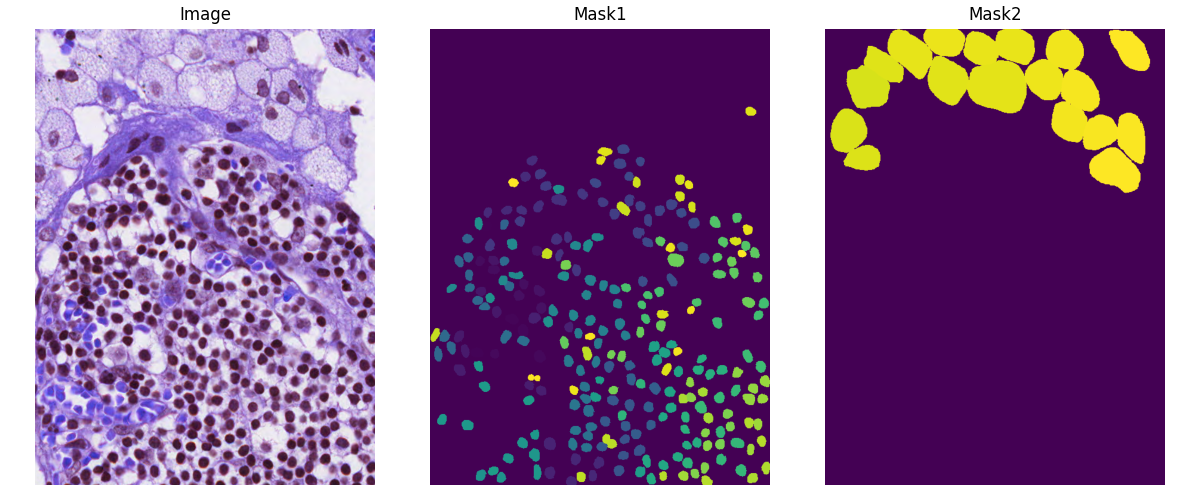
\includegraphics[width=0.95\linewidth]{assets/instance_segmentation.png}
  \caption{\textbf{Visualization of instance segmentation.} The image comes 
    from the provided dataset. The left image is the original image, and the
    right two images are the different classes in the image. The colors
    represent different instances of the same class.}
  \label{fig:instance-segmentation}
\end{figure}

\subsection{Mask R-CNN}

Mask R-CNN~\cite{MaskRCNN} is an advanced deep learning model for instance
segmentation that extends Faster R-CNN~\cite{FasterRCNN}  by adding a branch
for predicting segmentation masks. While Faster R-CNN detects object bounding
boxes and classifies them, Mask R-CNN also generates a pixel-level mask for
each detected object. It achieves this by adding a parallel fully convolutional
network (FCN)~\cite{FCN} head to predict masks and using RoIAlign instead of
RoIPool for better spatial alignment. This makes Mask R-CNN more accurate for
precise object delineation.


\subsection{Data Augmentation}

Data augmentation is a technique used in computer vision to improve model
generalization by applying transformations like rotation, cropping, and
distortion to training images, especially when the dataset is small. It helps
to create variations of the training data, making the model more robust to
different conditions and reducing overfitting. Furthermore, Albumentations~\cite{info11020125}
says that grid distortion and elastic transform, two types of non-linear
distortions, are helpful for medical images.  Such a method may be suitable
for this task.

% --------------------------- Method ---------------------------

\section{Method}
\label{sec:method}

\subsection{Data Preprocessing and Augmentation}

The training dataset contains 209 images with masks. It is split into training
and validation set with a ratio of 8:2.

Some data augmentations are applied to the training set. These include:
\begin{itemize}
  \setlength\itemsep{0pt}
  \item Random horizontal flip
  \item Random color jitter
  \item Random affine transformation
  \item Elastic Transform
  \item Random Gaussian blur or Gaussian noise
\end{itemize}

The elastic Transform is a non-linear distortion that randomly deforms the image
by applying a random displacement field. It is implemented by the
\texttt{albumentations} library.

\subsection{Model Architecture}

The backbone remains the same as the original implementation, which is ResNet-50.
I've also tried ResNet-101 and ResNeXt-50~\cite{ResNeXt}, but unlike previous tasks,
they do not improve the performance in this task. For the experiment result and
analysis, please refer to \cref{sec:other-exp}.

The backbone is frozen except for the last layer since the customized dataset is
small compared to the ImageNet dataset, which is used to pretrain the backbone.
It may be hard to train the whole backbone on a small dataset. The last layer is
unfrozen to still allow the model to learn the features of the dataset.

The architecture of RPN remains unchanged. After region proposals are generated
and refined (by NMS) by RPN, they are projected onto the shared feature map
and passed through a RoI Align layer to produce fixed-size feature vectors.
These vectors are then fed into two branches: one for object detection and
one for instance segmentation. The object detection branch is like Faster R-CNN,
while the instance segmentation branch is a fully convolutional network (FCN)
that predicts a binary mask for each object.

\subsection{Optimization}

For optimization, AdamW~\cite{AdamW} is used with an initial learning rate of 5e-5.
A cosine annealing scheduler~\cite{CosineAnnealing} dynamically adjusts the learning
rate throughout training. The training process is conducted with a batch size of 2
over 50 epochs. The dataset contains roughly 168 training images, 41 validation
images, and 101 test images. The best-performing model is selected based on AP50,
which is calculated from COCOeval. The model is trained on a single NVIDIA GeForce
RTX 4090 GPU in about 2 hours.

\subsection{Hyperparameters}

\noindent The hyperparameter details are listed below:
\begin{itemize}
  \setlength\itemsep{0pt}
  \item Learning rate: 5e-5
  \item Optimizer: AdamW
  \item Scheduler: CosineAnnealingLR
  \item Batch Size: 2
  \item Epochs: 50
\end{itemize}

\section{Results}

In this section, I compare the performance of each component in the model.
The details of each method are listed:
\begin{itemize}
  \setlength\itemsep{0pt}
  \item Res50: ResNet-50 pretrained on ImageNet without any tricks but only freeze
    the whole backbone.
  \item Aug.: The same setting as Res50, but perform data augmentation excluding
    elastic transform.
  \item Elastic: Perform the same data augmentation but including elastic transform.
  \item Partial: Partial fine-tuning ResNet-50, which means unfreezing the last layer
    of the ResNet-50.
\end{itemize}

The results are shown in \cref{tab:result}. The validation AP50 curve and training
loss curve are shown in \cref{fig:val-ap50} and \cref{fig:train-loss}, respectively.
The training loss is calculated by summing the loss of the object detection and
instance segmentation branches. Even though some methods do not surpass Res50 in
validation and public testing, they all perform better than Res50 in private testing.
Thus, they are all selected in the final model.

Moreover, I find that adding elastic transform may not improve the performance
much. It has less than 0.01 improvement in private testing and even worse in
validation and public testing. This is different from what Albumentations
says. I guess it is because the object in the dataset is small and
shape-dependent. The elastic transform may adjust the object too much, or even
not proper for this dataset.

\begin{table}[h]
  \centering
  \begin{tabular}{lccc}
    \toprule
    \multicolumn{1}{c}{\textbf{Method}} & \textbf{Val}              & \textbf{Test pub.}          & \textbf{Test priv.}       \\
    \midrule
    Res50                               & 0.4699                    & 0.3640                      & 0.3108                    \\
    \hdashline
    Aug.                                & \tbbgred 0.4555           & \tbbgred 0.3532             & \tbbgblue 0.3663          \\
    Elastic                             & \tbbgred 0.4392           & \tbbgred 0.3383             & \tbbgblue 0.3671          \\
    Partial                             & \tbbgblue \textbf{0.4912} & \tbbgred 0.3271             & \tbbgblue 0.3608          \\       
    Partial + Aug.                      & \tbbgblue 0.4906          & \tbbgred \textbf{0.3606}    & \tbbgblue 0.3827          \\
    Partial + Elastic                   & \tbbgblue 0.4855          & \tbbgred 0.3391             & \tbbgblue \textbf{0.3853} \\
    \bottomrule
  \end{tabular}
  \caption{\textbf{The AP50 results of different methods.} ``Val" refers to
    validation AP50. ``Test pub." and ``Test priv." refer to public and
    private test set AP50, respectively. Res50 is treated as the baseline.
    If the value is higher than Res50, it is highlighted in blue, or it will
    be in red. The highest values in each column are also highlighted in bold.
  }
  \label{tab:result}
\end{table}



\begin{figure}[h]
  \centering
  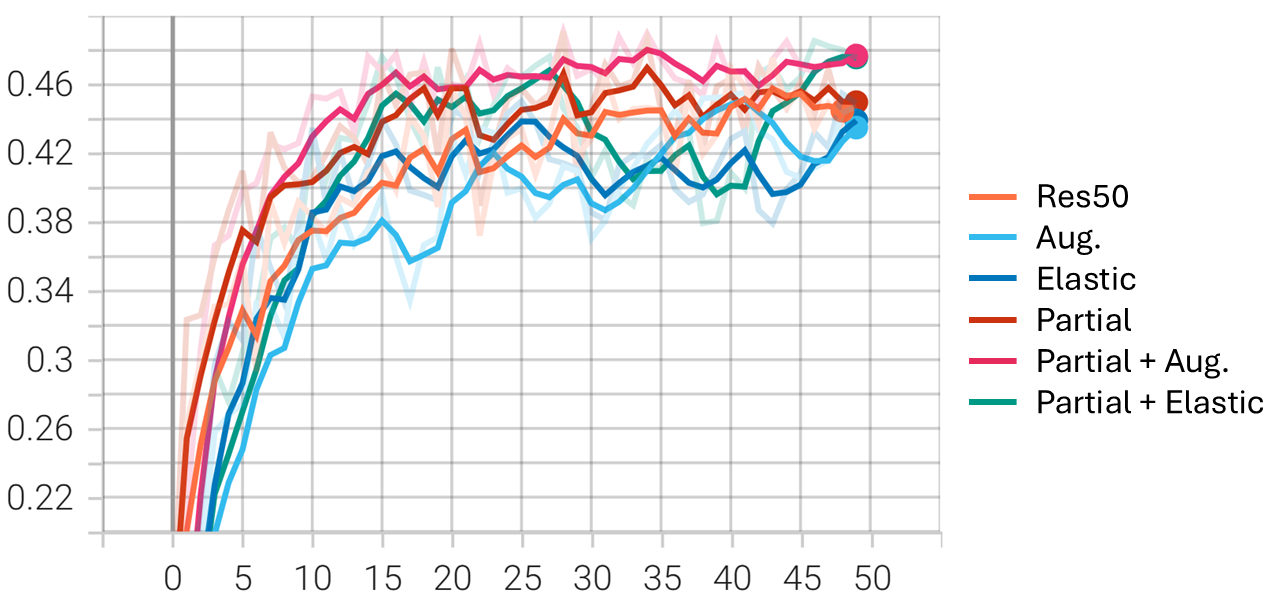
\includegraphics[width=0.95\linewidth]{assets/val_ap50.png}
  \caption{\textbf{Validation AP50 curve of different method.}}
  \label{fig:val-ap50}
\end{figure}

\begin{figure}[h]
  \centering
  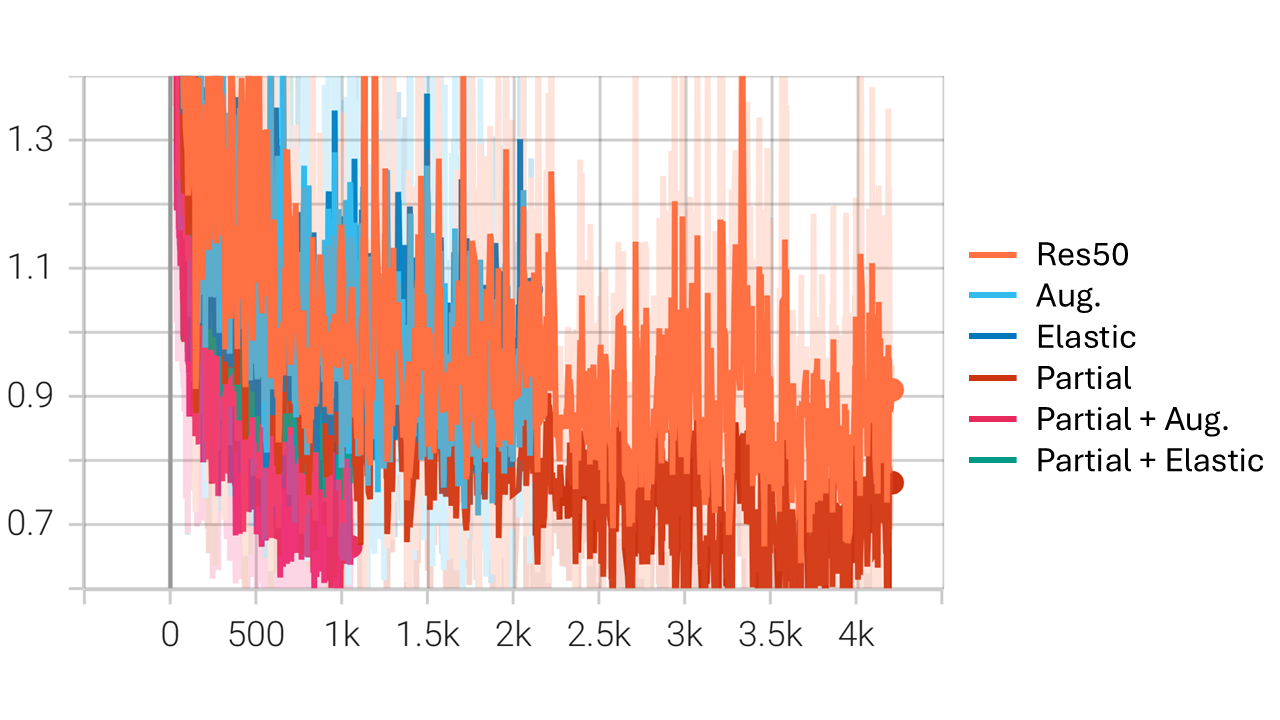
\includegraphics[width=0.95\linewidth]{assets/train_loss.png}
  \caption{\textbf{Training loss curve of different method.}}
  \label{fig:train-loss}
\end{figure}

% ----------------------- Other Experiments -----------------------

\section*{Other Experiments}
\label{sec:other-exp}

\subsection*{The Selection of Backbone}

I've conducted experiments with different backbones, including ResNet-50,
ResNet-101 and ResNeXt-50. The entire backbone is frozen, treating these
models as feature extractors. The results are shown in \cref{fig:exp-backbone}.
While ResNet-101 and ResNeXt-50 are more powerful than ResNet-50, they do not
improve the performance in this task. I guess it is because the pretrained
weights of ResNet-50 are specially trained on instance segmentation task. While
ResNet-101 and ResNeXt-50 are not, they are just trained on their original image
classification task. Therefore, utilizing ResNet-50 with well-pretrained weights
is more suitable for this task.

\begin{figure}[h]
  \centering
  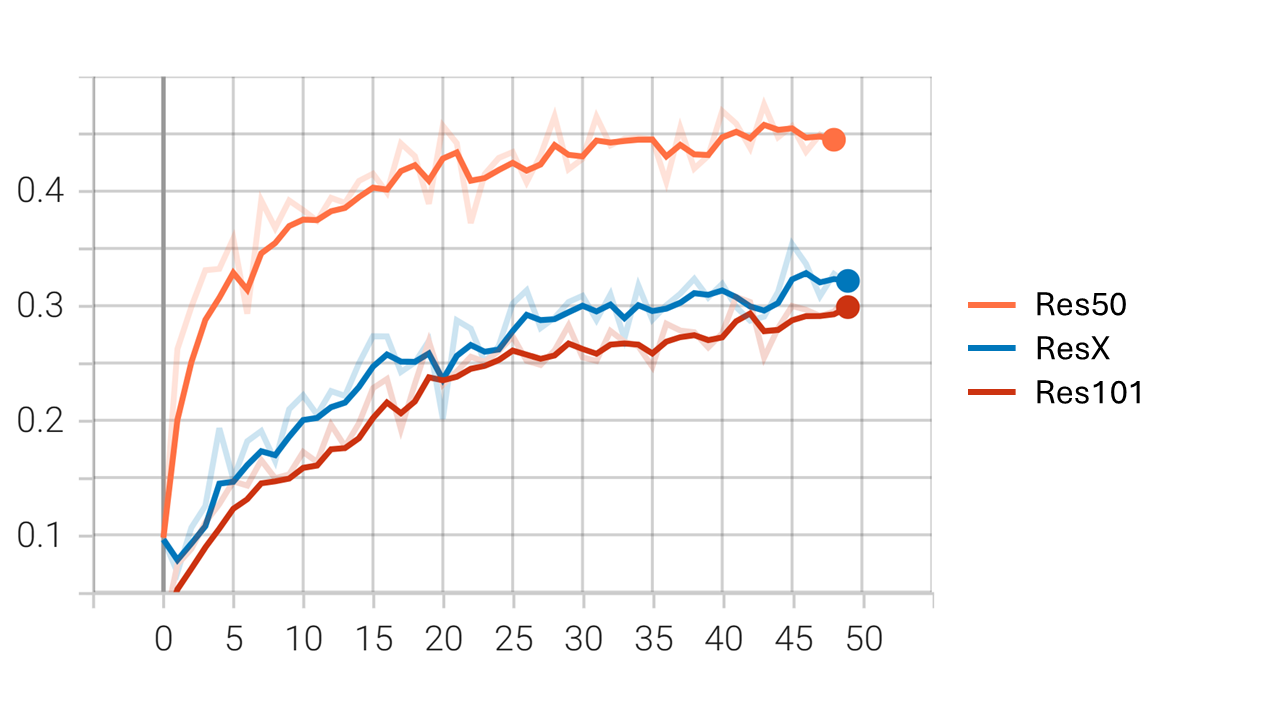
\includegraphics[width=0.95\linewidth]{assets/exp_backbone_ap50.png}
  \caption{\textbf{The AP50 results of different backbones.}}
  \label{fig:exp-backbone}
\end{figure}

\subsection*{Restart Strategy}

In previous homework, restart strategy always improves the performance
of the model. However, in this task, it does not always work. I applied it
to Mask R-CNN with backbone as ResNet-50 but it turns out a degradation
of the performance. The experiment result is shown in \cref{tab:restart}.
The model is trained with the same hyperparameters and data augmentations,
the whole backbone is frozen as well. The only difference is the restart
strategy. My guess is that the dataset is too small, once the model is
restarted, it may not have enough data to learn again.

\begin{table}[h]
  \centering
  \begin{tabular}{lccc}
    \toprule
    \multicolumn{1}{c}{\textbf{Method}}   & \textbf{Val}    & \textbf{Test pub.} & \textbf{Test priv.} \\
    \midrule
    Res50                                 & \textbf{0.4699} & \textbf{0.3640}    & 0.3108              \\
    Res50 w/ restart                      & 0.4411          & 0.3471             & \textbf{0.3142}     \\
    \bottomrule
  \end{tabular}
  \caption{\textbf{The AP50 results of applying restart.} The definition of the
    term is the same as \cref{tab:result}. The highest values in each
    column are highlighted in bold.
  }
  \label{tab:restart}
\end{table}

\subsection*{Freezing Model}

In this task, only about 180 images are used for training. The backbone
is pretrained on ImageNet, which contains about 1.2 million images.
Fine-tuneing the whole backbone may not work well due to the small dataset.
In my guess, I think leveraging the knowledge from ImageNet is more suitable
for feature extraction. Therefore, I test the performance of full fine-tuning,
freezing the backbone, and partial fine-tuning (unfreeze the last layer).
The experiment result is shown in \cref{tab:exp-freeze}. It shows that the
partial fine-tuning works the best, while full fine-tuning has a significant
poor performance.

\begin{table}[h]
  \centering
  \begin{tabular}{lccc}
    \toprule
    \multicolumn{1}{c}{\textbf{Method}} & \textbf{Val}    & \textbf{Test pub.} & \textbf{Test priv.} \\
    \midrule
    Full fine-tuning                     & 0.3460          & \textbf{0.3640}    & 0.3108              \\
    Freezing                            & 0.4699          & -                  & -                   \\
    Partial fine-tuning                  & \textbf{0.4912} & 0.3271             & \textbf{0.3608}     \\
    \bottomrule
  \end{tabular}
  \caption{\textbf{The results of freezing the model.} The highest values
  in each column are highlighted in bold. ``Freezing" has
  significantly worse AP50, so I do not evaluate it on the test set. 
  }
  
  \label{tab:exp-freeze}
\end{table}


%%%%%%%%% REFERENCES %%%%%%%%%
{\small
\bibliographystyle{ieee_fullname}
\bibliography{egbib}
}

\end{document}